\documentclass[Lecture.tex]{subfiles}
\begin{document}
\section{1.1: Functions}

\begin{frame}{Definition}
  \begin{defn}
    \begin{itemize}
    \item<1->
      A {\it function} is a rule that takes certain values as inputs and assigns to each input {\bf exactly one} output.
    \item<2->
      The set of all possible inputs is called the {\it domain} of the function.
    \item<3->
      The set of all possible outputs is called the {\it range} of the function.
    \end{itemize}
  \end{defn}
  \pause
  \only<4->{Notation:
  A function named $f$ that takes as input the {\it independent variable}, $x$, and outputs the {\it dependent variable}, $y$, is written as
  $$y = f(x).$$}
\end{frame}

\begin{frame}{Example (Discrete Function)}
  \onslide<1->{Given any two sets we can define a function.}
  \onslide<2->{Say we have the sets
  $$D = \{1,2,3,4\}\ \text{and}\ R = \{5,6,7,8\}.$$}
  \onslide<3->{Define}
  \begin{multicols}{3}
      \begin{itemize}
      \item<3->
        f(1) = 6
      \item<4->
        f(2) = 5
      \item<5->
        f(3) = 8
      \item<6->
        f(4) = 7
      \end{itemize}
      \columnbreak
    \onslide<7->{
      \begin{tikzpicture}[
     >=stealth,
     bullet/.style={
       fill=black,
       circle,
       minimum width=1pt,
       inner sep=1pt
     },
     projection/.style={
       ->,
       thick,
       shorten <=2pt,
       shorten >=2pt
     },
     every fit/.style={
       ellipse,
       draw,
       inner sep=0pt
     }
   ]
     \foreach \y/\l in {1/4,2/3/,3/2,4/1}
       \node[bullet,label=left:$\l$] (a\y) at (0,\y) {};
 
     \foreach \y/\l in {1/8,2/7,3/6,4/5}
       \node[bullet,label=right:$\l$] (b\y) at (4,\y) {};
 
     \node[draw,fit=(a1) (a2) (a3) (a4),minimum width=2cm] {} ;
     \node[draw,fit=(b1) (b2) (b3) (b4),minimum width=2cm] {} ;
 
     \onslide<7->{\draw[projection] (a1) -- (b2);}
     \onslide<8->{\draw[projection] (a2) -- (b1);}
     \onslide<9->{\draw[projection] (a3) -- (b4);}
     \onslide<10->{\draw[projection] (a4) -- (b3);}
   \end{tikzpicture}}
  \end{multicols}
\end{frame}

\begin{frame}{Example}
  The function $f(x) = x^2$ is a function.
  \begin{center}
    \begin{itemize}
    \item<2->
      The domain of $f$ is the set of all real numbers, $\R$.\\
    \item<3->
      The range of $f$ is the set of all non-negative real numbers,
      $$\left\{x \in \R \;\middle\vert\; 0 \leq x\right\}.$$
    \end{itemize}
  \end{center}
\end{frame}

\begin{frame}{Non-Example}
  The following depicts a non-function.
  \begin{center}
    \onslide<2->{
      \begin{tikzpicture}[
          >=stealth,
          bullet/.style={
            fill=black,
            circle,
            minimum width=1pt,
            inner sep=1pt
          },
          projection/.style={
            ->,
            thick,
            shorten <=2pt,
            shorten >=2pt
          },
          every fit/.style={
            ellipse,
            draw,
            inner sep=0pt
          }
        ]
        \foreach \y/\l in {1/4,2/3/,3/2,4/1}
        \node[bullet,label=left:$\l$] (a\y) at (0,\y) {};
        
        \foreach \y/\l in {1/8,2/7,3/6,4/5}
        \node[bullet,label=right:$\l$] (b\y) at (4,\y) {};
        
        \node[draw,fit=(a1) (a2) (a3) (a4),minimum width=2cm] {} ;
        \node[draw,fit=(b1) (b2) (b3) (b4),minimum width=2cm] {} ;
        
        \onslide<7->{\draw[projection] (a4) -- (b1);}
        \onslide<6->{\draw[projection] (a1) -- (b2);}
        \onslide<5->{\draw[projection] (a2) -- (b3);}
        \onslide<4->{\draw[projection] (a3) -- (b4);}
        \onslide<3->{\draw[projection] (a4) -- (b3);}
    \end{tikzpicture}}
  \end{center}
  \onslide<8->{The value $f(1)$ is not well-defined because it requires a choice: it could be either 6 or 8.}
\end{frame}

\subsection{Graphs}

\begin{frame}{Cartesian Plane}
  Recall that the {\it Cartesian plane} is the set of all pairs
  $$\R^2 = \left\{(x,y) \;\middle\vert\; x \in \R, y \in \R\right\}.$$
  \pause
  It can be depicted as 
  \begin{center}
    \begin{tikzpicture}
      \begin{axis}
        [
          width=3in,
          axis equal image,
          clip=false,
          axis lines=middle,
          xmin=-5,
          xmax=5,
          ymin=-5,
          ymax=5,
          restrict y to domain=-5:5,
          xtick={\empty},
          ytick={\empty},
          axis line style={latex-latex},
          xlabel=$x$,
          ylabel=$y$,
          xlabel style={at={(ticklabel* cs:1)},anchor=north west},
          ylabel style={at={(ticklabel* cs:1)},anchor=south west},
        ]
      \end{axis}
    \end{tikzpicture}
  \end{center}
\end{frame}

\begin{frame}{Graph of a Function}
  \begin{defn}
    The graph of a real-valued function, $f$, with domain $D \subseteq \R$ is the set of pairs
    $$\left\{(x, f(x)) \;\middle\vert\; x \in D\right\} \subseteq \R^2.$$
    It can be drawn on the Cartesian plane.
  \end{defn}
\end{frame}

\begin{frame}{Example}
  The function $f(x) = x$ has 
  \begin{itemize}
    \item<2->
      Domain all real numbers, $\R$,
    \item<3->
      Range all real numbers, $\R$,
    \item<4->
      Graph $\left\{(x,x) \;\middle\vert\; x \in \R\right\}$,
      \onslide<5->
      \begin{center}
        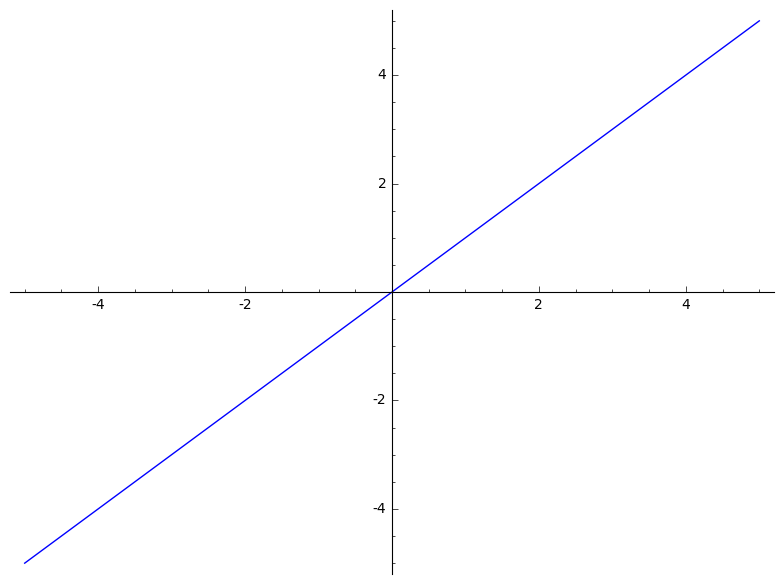
\includegraphics[scale=0.25]{idGraph}
      \end{center}
  \end{itemize}
\end{frame}


\begin{frame}{Increasing/Decreasing Functions}
  \begin{defn}
    Let $f$ be a function and let $[a,b]$ be an interval contained in the domain of $f$.
    We say $f$ is
    \begin{itemize}
      \item<2->
        {\it increasing on [a,b]} if $f(x_1) < f(x_2)$ whenever $a \leq x_1 < x_2 \leq b$,
      \item<3->
        {\it decreasing on [a,b]} if $f(x_2) < f(x_1)$ whenever $a \leq x_1 < x_2 \leq b$.
    \end{itemize}
    \onslide<4->
    We say that $f$ is increasing/decreasing if it is increasing/decreasing on its entire domain.
  \end{defn}
\end{frame}

\begin{frame}{Example}
  \begin{center}
    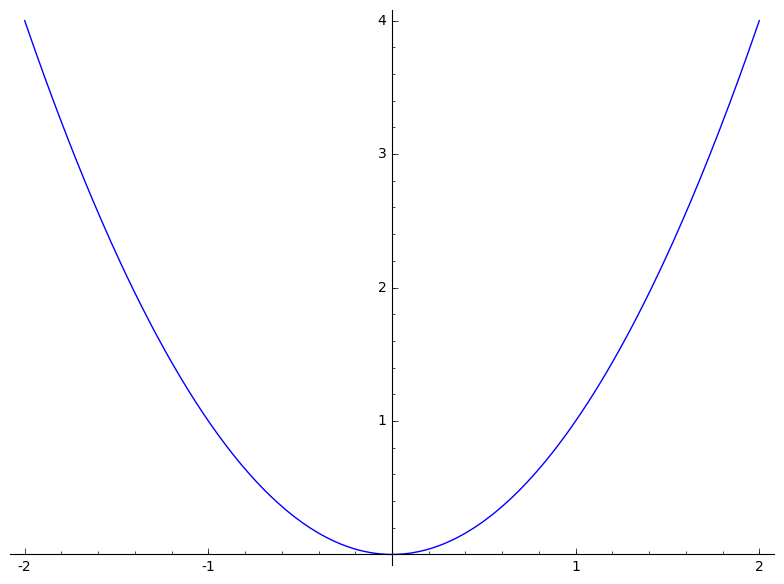
\includegraphics[scale=0.25]{parabola}
  \end{center}
  \begin{itemize}
  \item<2->
    Increasing on: \onslide<3->{$(0,\infty)$}
  \item<2->
    Decreasing on: \onslide<4->{$(-\infty,0)$}
  \end{itemize}
\end{frame}

\begin{frame}{Example}
  \begin{multicols}{2}
    
  \begin{center}
    Increasing\\
    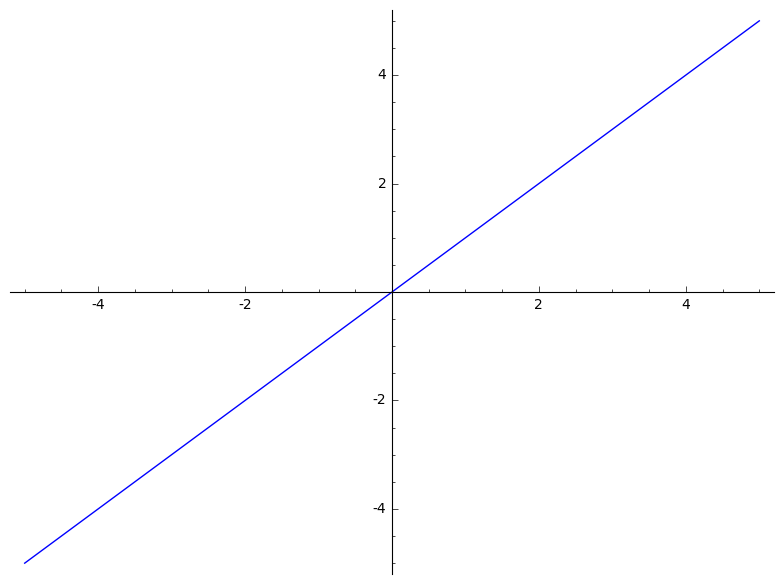
\includegraphics[scale=0.25]{idGraph}
  \end{center}
  \columnbreak
  \pause
  \begin{center}
    Decreasing\\
    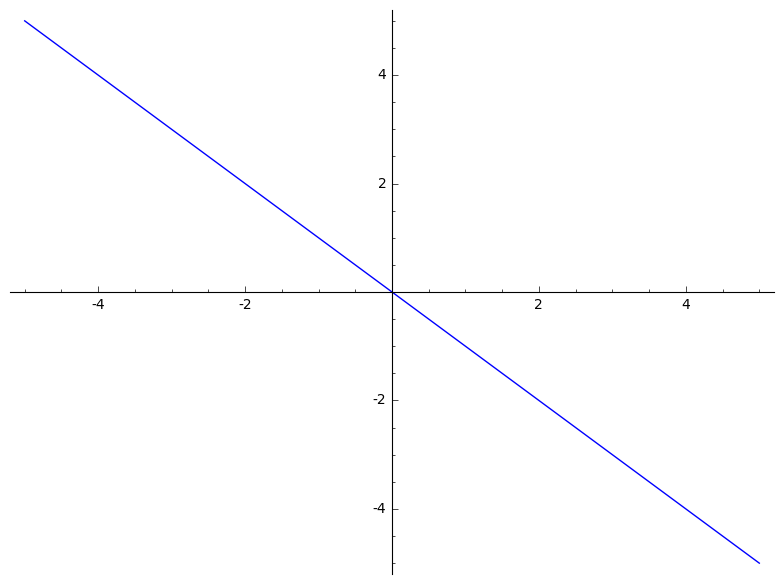
\includegraphics[scale=0.25]{negIdGraph}
  \end{center}
  \end{multicols}
\end{frame}

\begin{frame}{Intercepts}
  \begin{defn}
    Let $f$ be a function of a real variable, $x$.
    \begin{itemize}
      \item<2->
        The {\it $x$-intercepts} are the points $(x,0)$ on the graph.
      \item<3->
        The {\it $y$-intercept} is the point $(0,f(0))$ on the graph.
    \end{itemize}
  \end{defn}
\end{frame}

\begin{frame}{Example}
  Let $f(x) = x - 1$.\\
  \pause
  The $y$-intercept is
  $$(0,f(0)) = (0, 0 - 1) = (0,-1).$$\\
  \pause
  The $x-intercept$ is $(1,0)$:
  $$f(1) = 1 - 1 = 0.$$\\
  \pause
  \begin{center}
    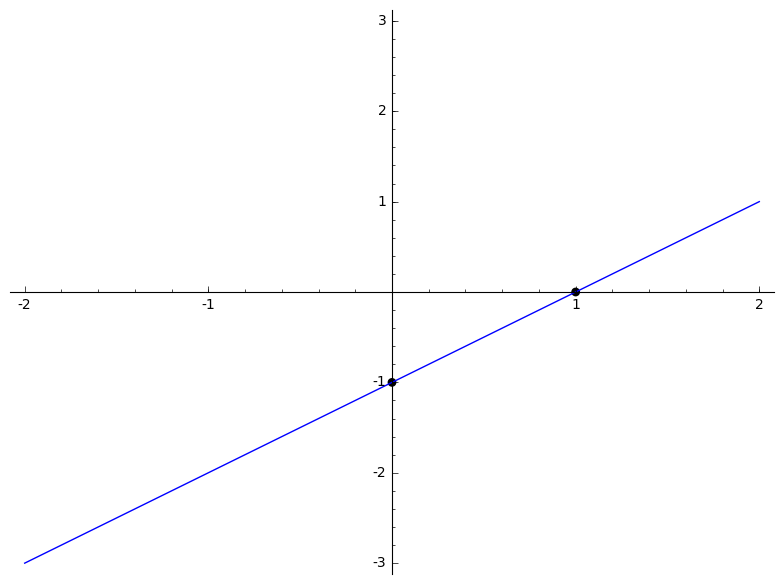
\includegraphics[scale=0.25]{intercepts}
  \end{center}
\end{frame}
\end{document}
